% =============================================================================
\section{Analyse par instance}
\label{sec:analysis}
% =============================================================================

Pour chaque instance, nous présentons une comparaison visuelle des
trajectoires obtenues par les trois méthodes (CMA-ES, DE, GA) et une
discussion des résultats.

% ---------- prob1 ----------
\subsection{\texttt{prob1} — Trajectoire diagonale, 5~obstacles épars}

\begin{figure}[H]
\centering
\begin{subfigure}[b]{0.32\textwidth}
  \centering
  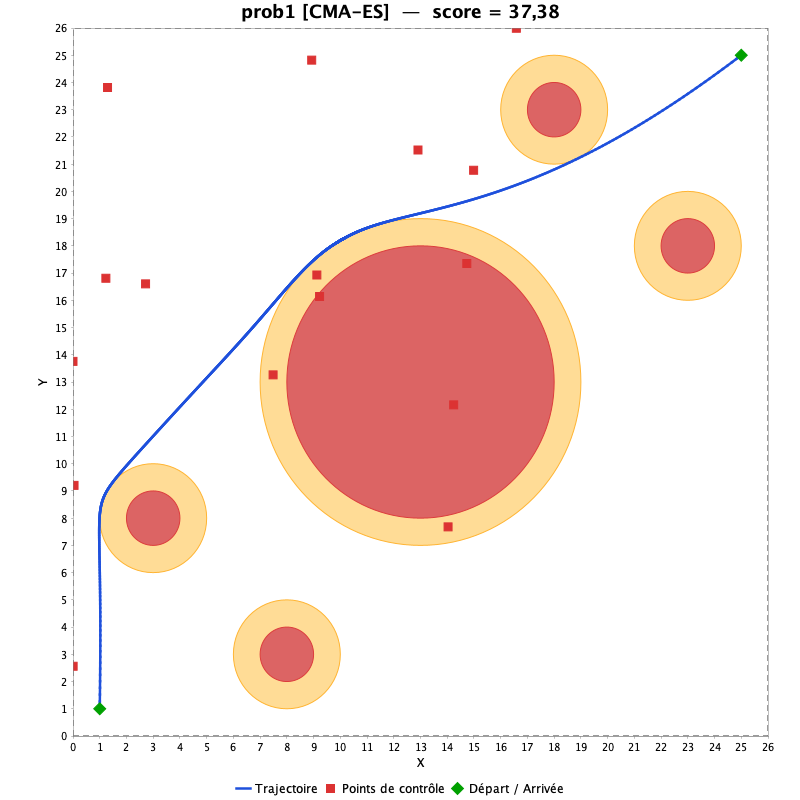
\includegraphics[width=\textwidth]{figures/path_prob1_cmaes.png}
  \caption{CMA-ES}
\end{subfigure}
\hfill
\begin{subfigure}[b]{0.32\textwidth}
  \centering
  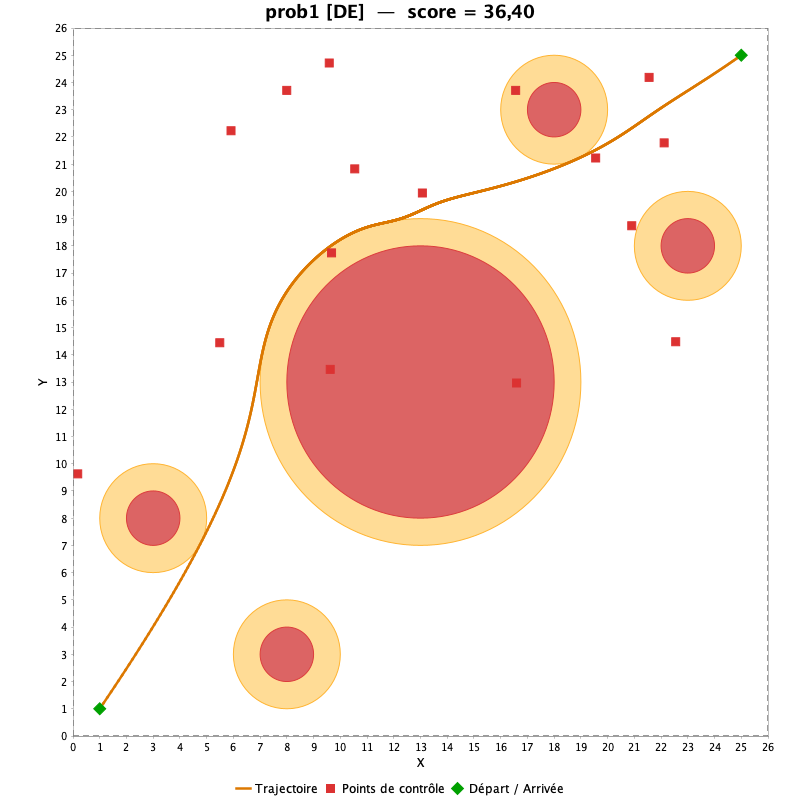
\includegraphics[width=\textwidth]{figures/path_prob1_de.png}
  \caption{DE}
\end{subfigure}
\hfill
\begin{subfigure}[b]{0.32\textwidth}
  \centering
  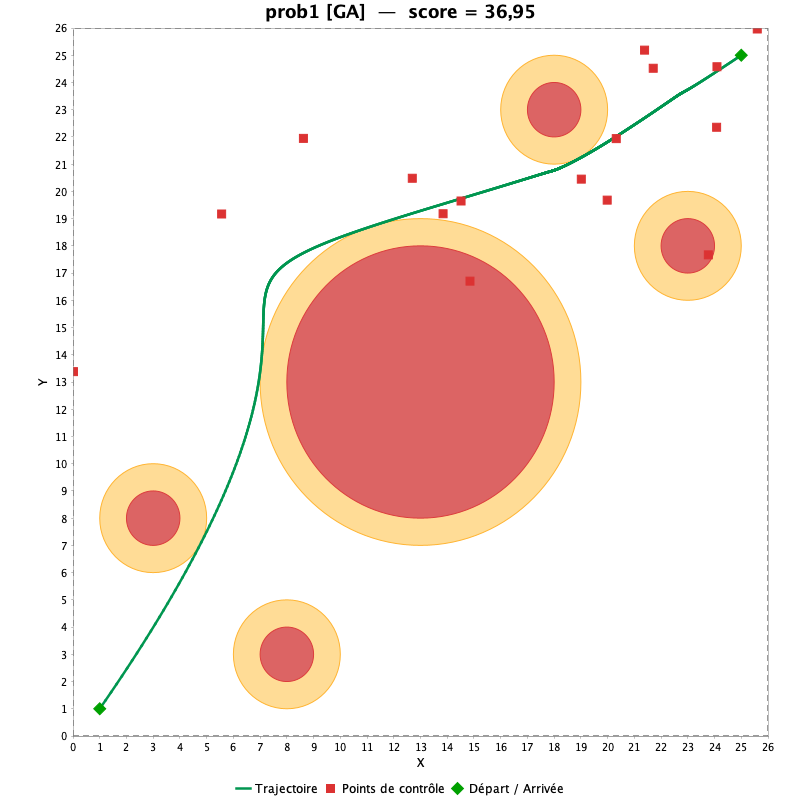
\includegraphics[width=\textwidth]{figures/path_prob1_ga.png}
  \caption{GA}
\end{subfigure}
\caption{Trajectoires optimisées pour \texttt{prob1} ($d=32$, 5~obstacles).}
\label{fig:prob1}
\end{figure}

\emph{Analyse.}  Avec $d = 32$ (16~points de contrôle), cette instance offre
une grande liberté de placement.  CMA-ES produit une trajectoire diagonale
quasiment optimale, exploitant l'adaptation de la covariance pour aligner les
$x$ et $y$ de façon corrélée.  DE et GA trouvent des chemins légèrement plus
longs ou présentant des ondulations inutiles, signe d'une convergence
incomplète dans l'espace $\mathbb{R}^{32}$.  Le score de CMA-ES ($\approx 37{,}4$)
est proche de la longueur euclidienne du chemin le plus court contournant les
obstacles.

% ---------- prob2 ----------
\subsection{\texttt{prob2} — Contournement d'un gros obstacle ($r = 9$)}

\begin{figure}[H]
\centering
\begin{subfigure}[b]{0.32\textwidth}
  \centering
  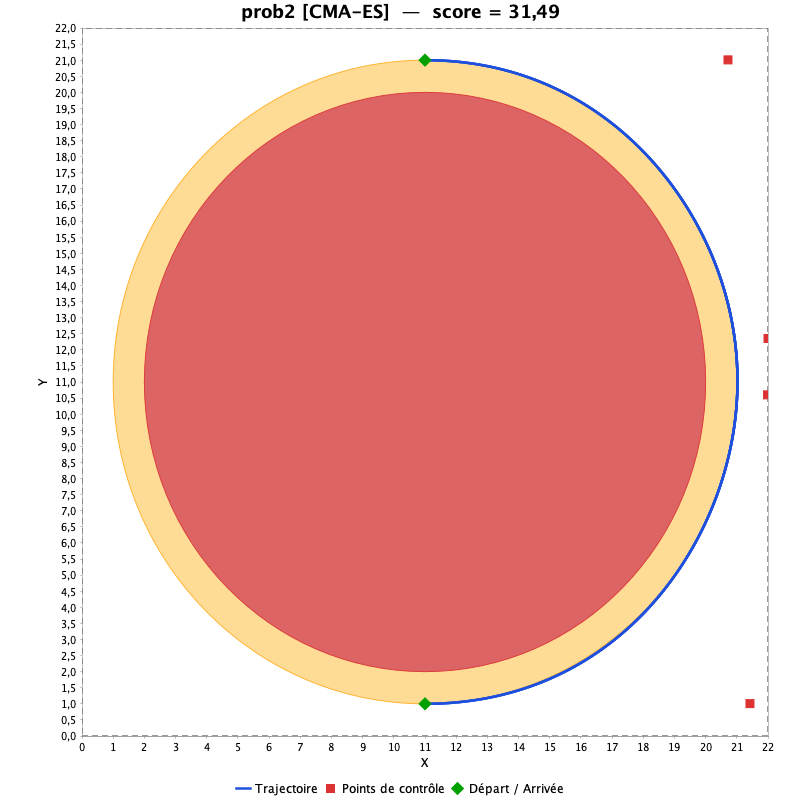
\includegraphics[width=\textwidth]{figures/path_prob2_cmaes.png}
  \caption{CMA-ES}
\end{subfigure}
\hfill
\begin{subfigure}[b]{0.32\textwidth}
  \centering
  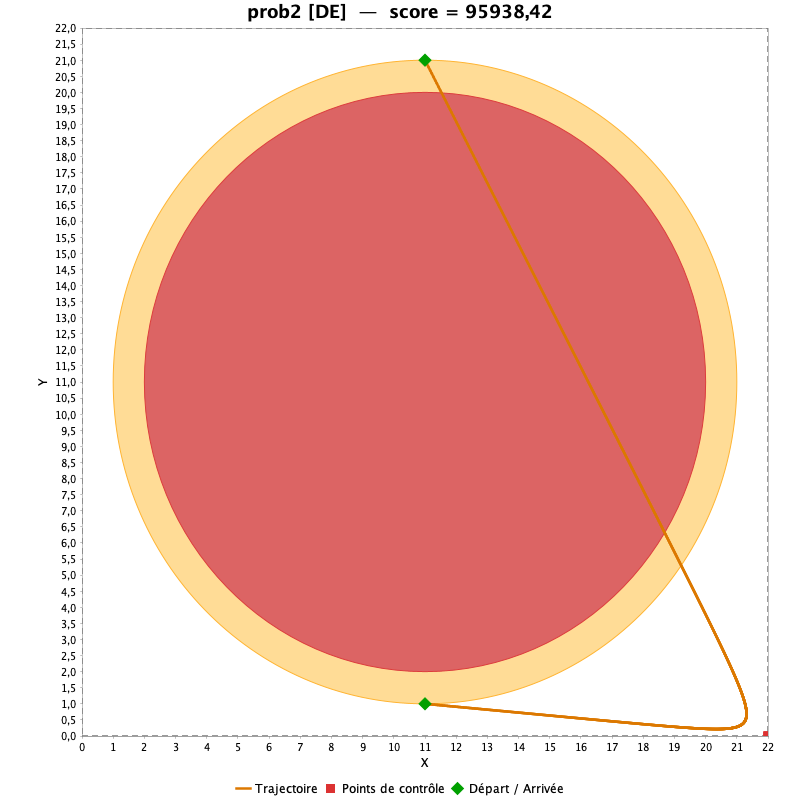
\includegraphics[width=\textwidth]{figures/path_prob2_de.png}
  \caption{DE}
\end{subfigure}
\hfill
\begin{subfigure}[b]{0.32\textwidth}
  \centering
  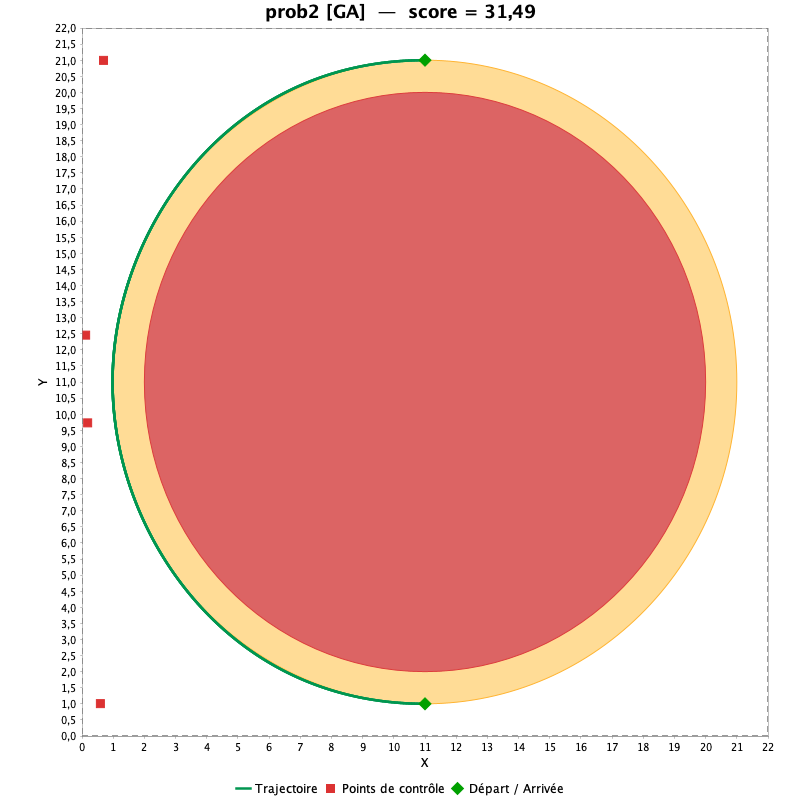
\includegraphics[width=\textwidth]{figures/path_prob2_ga.png}
  \caption{GA}
\end{subfigure}
\caption{Trajectoires optimisées pour \texttt{prob2} ($d=8$, 1~obstacle de rayon~9).}
\label{fig:prob2}
\end{figure}

\emph{Analyse.}  En faible dimension ($d = 8$), les trois méthodes convergent
vers des solutions de qualité comparable ($\approx 31{,}5$).  La trajectoire
est un arc de contournement quasi-circulaire autour de l'unique obstacle
central.  CMA-ES atteint le score optimal de façon quasi-déterministe (8/10
runs à $31{,}481$), ce qui confirme qu'il identifie efficacement l'optimum
global dans les espaces de faible dimension.

% ---------- prob3 ----------
\subsection{\texttt{prob3} — Slalom entre trois murs verticaux}

\begin{figure}[H]
\centering
\begin{subfigure}[b]{0.32\textwidth}
  \centering
  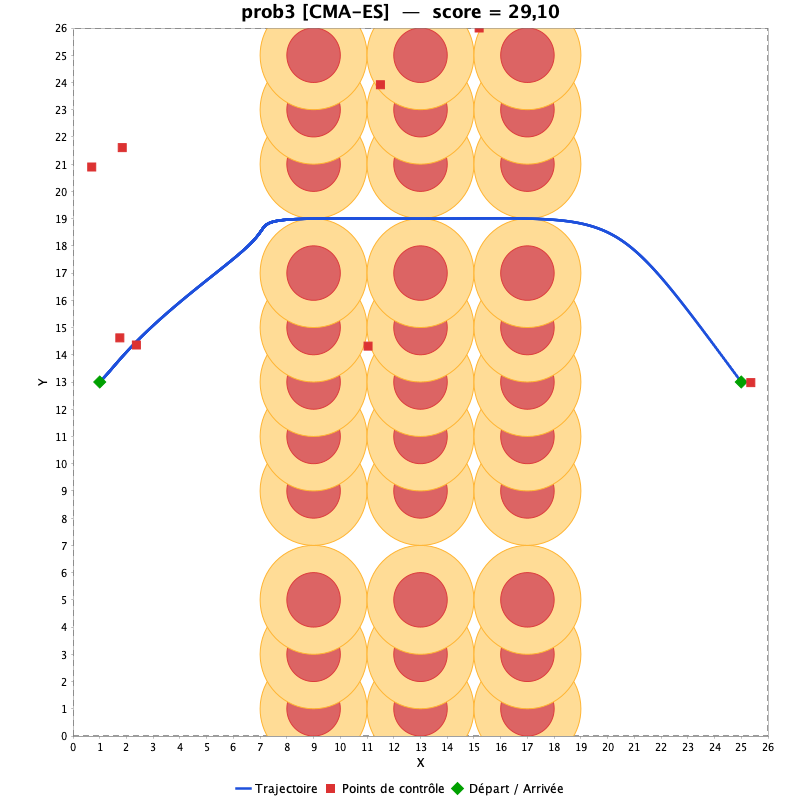
\includegraphics[width=\textwidth]{figures/path_prob3_cmaes.png}
  \caption{CMA-ES}
\end{subfigure}
\hfill
\begin{subfigure}[b]{0.32\textwidth}
  \centering
  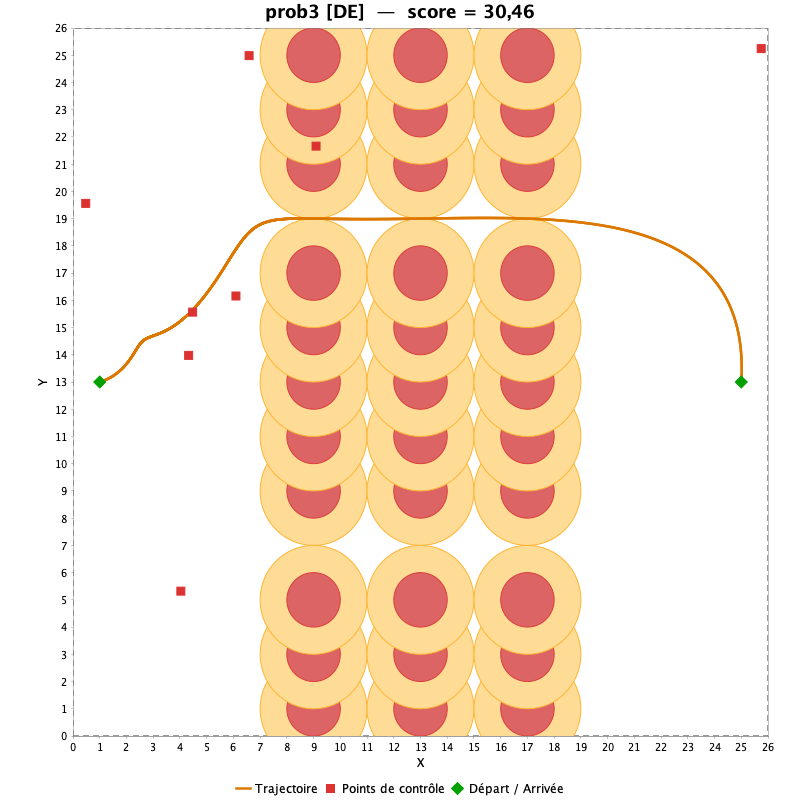
\includegraphics[width=\textwidth]{figures/path_prob3_de.png}
  \caption{DE}
\end{subfigure}
\hfill
\begin{subfigure}[b]{0.32\textwidth}
  \centering
  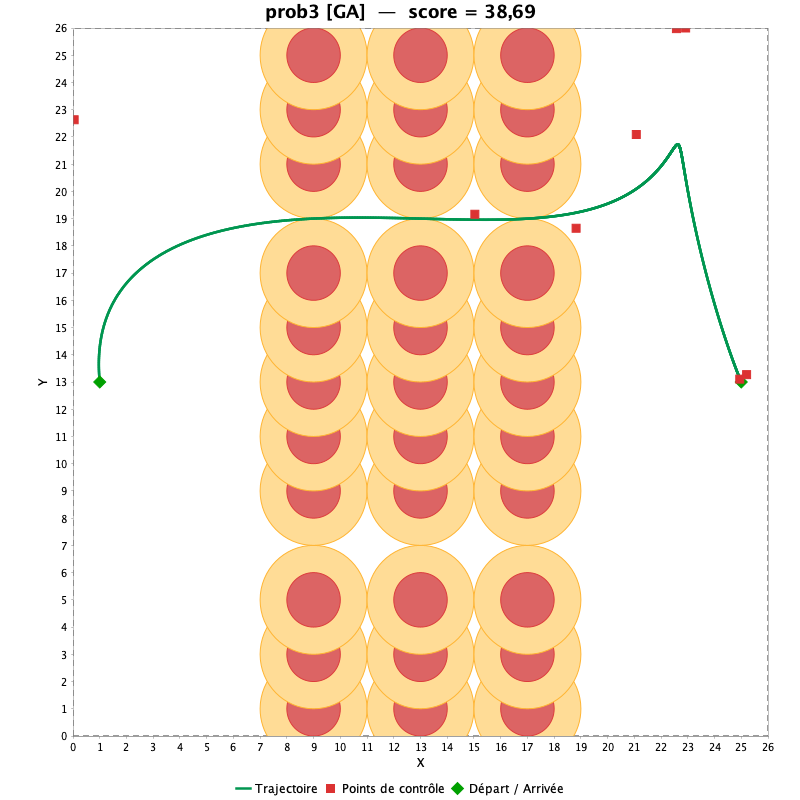
\includegraphics[width=\textwidth]{figures/path_prob3_ga.png}
  \caption{GA}
\end{subfigure}
\caption{Trajectoires optimisées pour \texttt{prob3} ($d=16$, 33~obstacles
         formant 3~murs verticaux).}
\label{fig:prob3}
\end{figure}

\emph{Analyse.}  Les 33~obstacles forment trois murs verticaux (à $x \approx
9, 13, 17$) percés de brèches.  La courbe de Bézier doit effectuer un
\emph{slalom} pour passer par ces brèches.  CMA-ES trouve un chemin fluide
($\approx 28{,}2$) en exploitant le seeding sinusoïdal qui pré-positionne les
points de contrôle dans des configurations ondulantes.  DE obtient $\approx
30{,}5$ et GA $\approx 38{,}7$ : la différence traduit l'incapacité du
croisement SBX (composante par composante) à capturer les corrélations entre
les abscisses et ordonnées successives des points de contrôle.

% ---------- prob4 ----------
\subsection{\texttt{prob4} — Labyrinthe en S}
\label{sec:prob4}

\begin{figure}[H]
\centering
\begin{subfigure}[b]{0.32\textwidth}
  \centering
  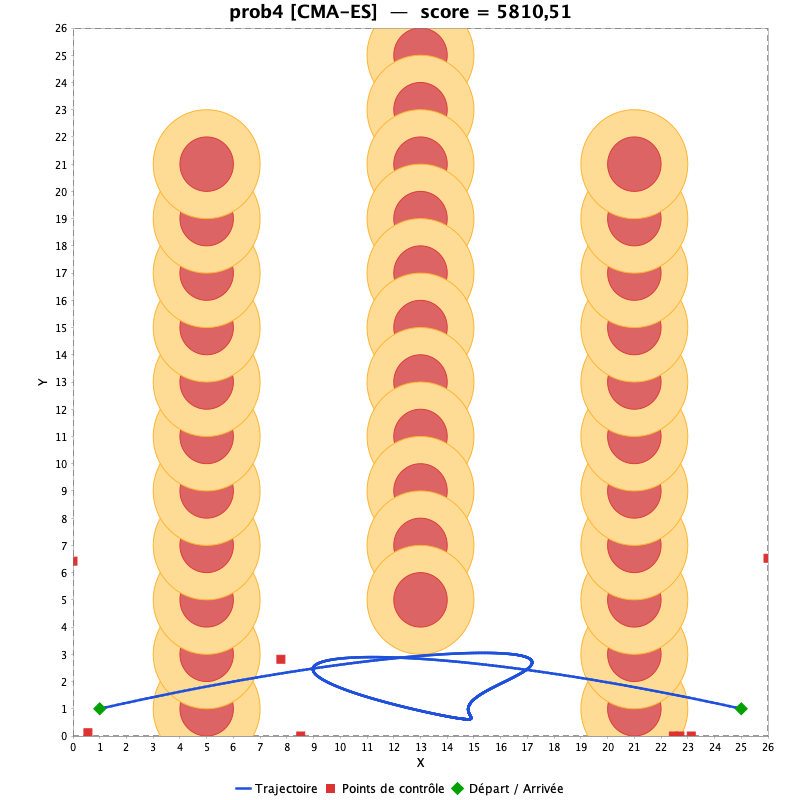
\includegraphics[width=\textwidth]{figures/path_prob4_cmaes.png}
  \caption{CMA-ES}
\end{subfigure}
\hfill
\begin{subfigure}[b]{0.32\textwidth}
  \centering
  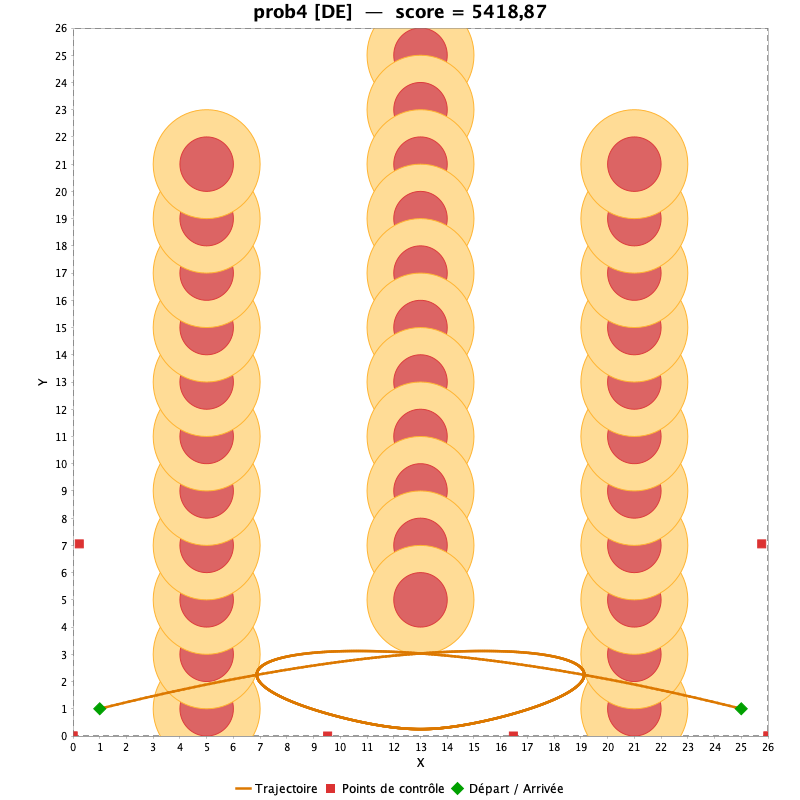
\includegraphics[width=\textwidth]{figures/path_prob4_de.png}
  \caption{DE}
\end{subfigure}
\hfill
\begin{subfigure}[b]{0.32\textwidth}
  \centering
  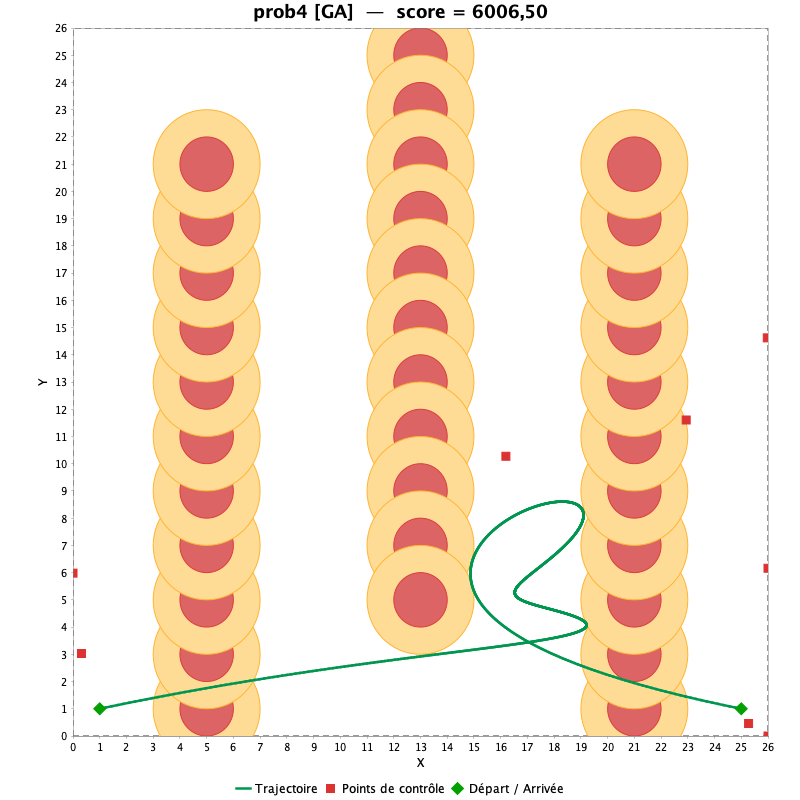
\includegraphics[width=\textwidth]{figures/path_prob4_ga.png}
  \caption{GA}
\end{subfigure}
\caption{Trajectoires optimisées pour \texttt{prob4} ($d=16$, 33~obstacles,
         labyrinthe en S).}
\label{fig:prob4}
\end{figure}

\emph{Analyse.}  \texttt{prob4} est le problème le plus difficile. Trois murs
d'obstacles ($x \approx 5, 13, 21$) bloquent le passage avec des brèches
alternées : brèche en \emph{haut} pour les murs~1 et~3 ($y > 22$), brèche en
\emph{bas} pour le mur~2 ($y < 4$).  Le chemin optimal exige un profil en S
(monter → traverser → descendre → traverser → remonter → redescendre) que la
courbe de Bézier de degré~10 ne peut pas représenter de manière précise.

\paragraph{Exploitation de la vitesse paramétrique.}
Une analyse diagnostique approfondie (évaluation de 500\,000 solutions
aléatoires, recherche exhaustive sur grille) a montré que CMA-ES découvre une
stratégie inattendue : en plaçant les points de contrôle aux \emph{frontières
du domaine} ($x = 0$ ou $x = 26$), la courbe de Bézier ``accélère''
paramétriquement dans les zones d'obstacles, réduisant le nombre de points
d'échantillonnage (parmi les 1\,000) qui tombent dans les zones de pénalité.
C'est pourquoi les graines de type « regroupements aux frontières »
(section~\ref{sec:seeding}) ont été ajoutées.

\paragraph{Résultats.}
Sur 10~runs, 4 descendent sous 3\,400 (minimum : 2\,931), là où les solutions
purement aléatoires plafonnent à $\approx 7\,500$.  Les 6~autres runs restent
autour de 5\,500--5\,800, piégés dans une configuration moins favorable.  Cette
forte variance ($\sigma \approx 1\,272$) reflète la \textbf{multi-modalité
extrême} de cette instance et constitue une \emph{limitation intrinsèque de
l'encodage} par courbe de Bézier unique, et non de l'algorithme en lui-même.
